\section{Introduzione}
Data la straordinarietà degli eventi che erano in corso dal punto di vista sanitario nel nostro paese si è reso necessario svolgere gran parte del lavoro in modalità a distanza e quindi senza la possibilità di testare il modello matematico appena ottenuto e i successivi risultati dovuti all'azione di controllo sul V.A.B.

Il lavoro quindi è stato svolto per la maggior parte sfruttando il tool \textit{Simulink} di Matlab il quale rappresenta, in poche parole, un risolutore di equazioni differenziali, le quali rappresentano la descrizione risultante del sistema che siamo andati a modellizzare.

Abbiamo così adottato una metodologia di lavoro basata su prototipi sempre più simili a quello che dovrebbe essere il sistema reale, lavorando step by step, partendo da modelli più semplici e aggiungendo via via features più complesse, in maniera da rendere il più aderente possibile il modello al sistema reale.

Si va ora ad analizzare la risposta del sistema al controllo ottenuto nei punti precedenti, per assicurarci, che quanto scritto sopra valga il più possibile, oltre che nella teoria, anche nella pratica.


\section{Simulazione in anello aperto}

Si è dunque proceduto, come primo approccio, a  simulare il sistema in anello aperto: senza controllo, come visto nella sezione ~\ref{sec:open_loop_analysis}, e come deduzione logica, non dovrebbe essere in grado di mantenere la posizione verticale (essendo essa un punto di equilibrio instabile).

La simulazione è stata portata avanti sul sistema non lineare, per il fatto che, nel sistema linearizzato risulta essere chiaro che, non appena ci si sposta dalla posizione di equilibrio intorno alla quale è stata realizzata la linearizzazione, il sistema non mostra il tipico andamento oscillante, ma va semplicemente a divergere, senza quindi fornire utili informazioni sul comportamento del sistema stesso.

\begin{figure}[H]
	\centering   	
	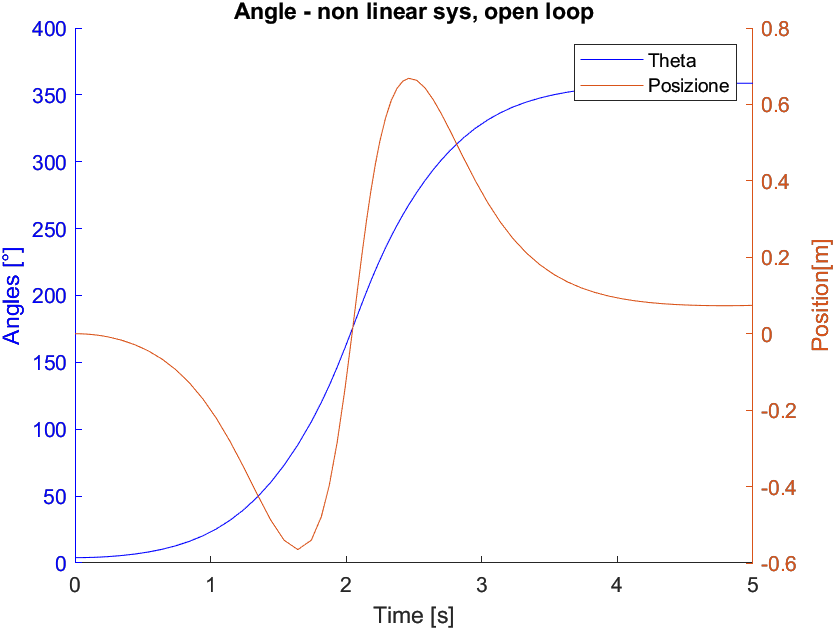
\includegraphics[width=0.6\textwidth]{Immagini/open_loop_response_non_linear.png}
	\caption{Risposta in anello aperto del sistema reale}
	\label{fig:open_loop_response_non_linear}
\end{figure}

Inoltre, essendo che nel sistema non sono stati modellizzati direttamente gli attriti, abbiamo che, partendo da una posizione verticale il veicolo autobilanciato continuerà a girare intorno all'asse delle ruote: questo è confermato dalle simulazioni in anello aperte fatte a differenti angoli di partenza (0 deg, 4 deg, 45 deg).

Come si vede nelle figure ~\ref{fig:angle_theta}, partendo da una posizione di 45 deg, il V.A.B. non è in grado di compiere una rotazione completa, poichè l'energia non è sufficiente per permettergli di passare dalla posizione verticale.

\begin{figure}[H]
	\centering
	\subfloat[][\emph{$\theta = 0deg$}]
	{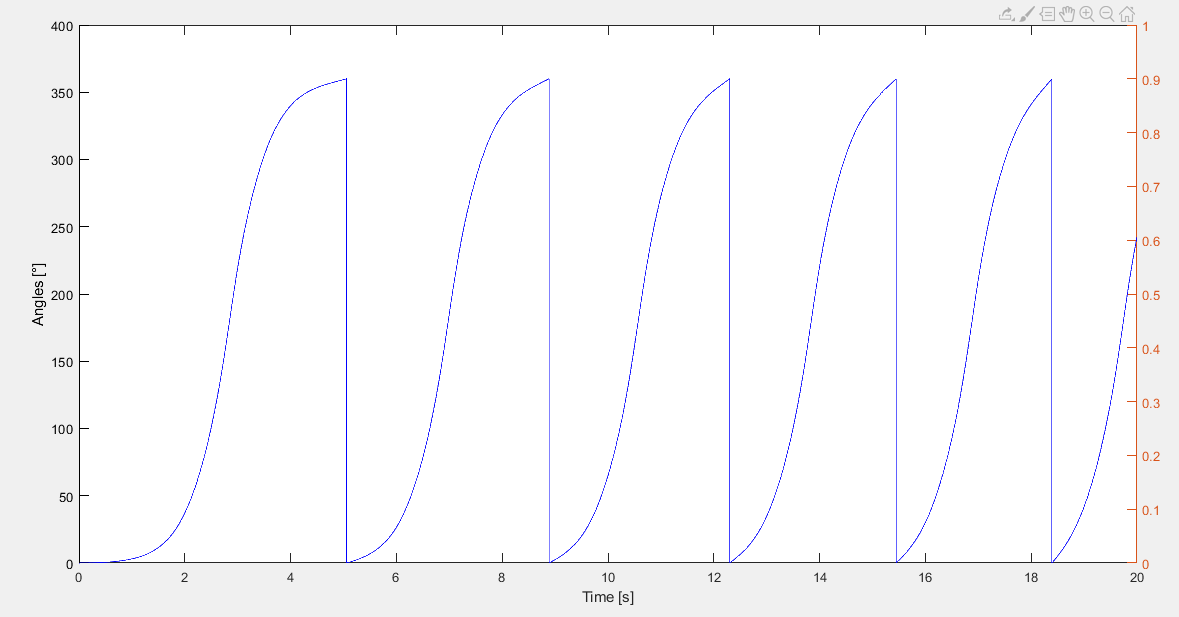
\includegraphics[width=.45\textwidth]{Immagini/open_loop_response_angle_clamped.png}} \quad
	\subfloat[][\emph{$\theta = 4deg$}]
	{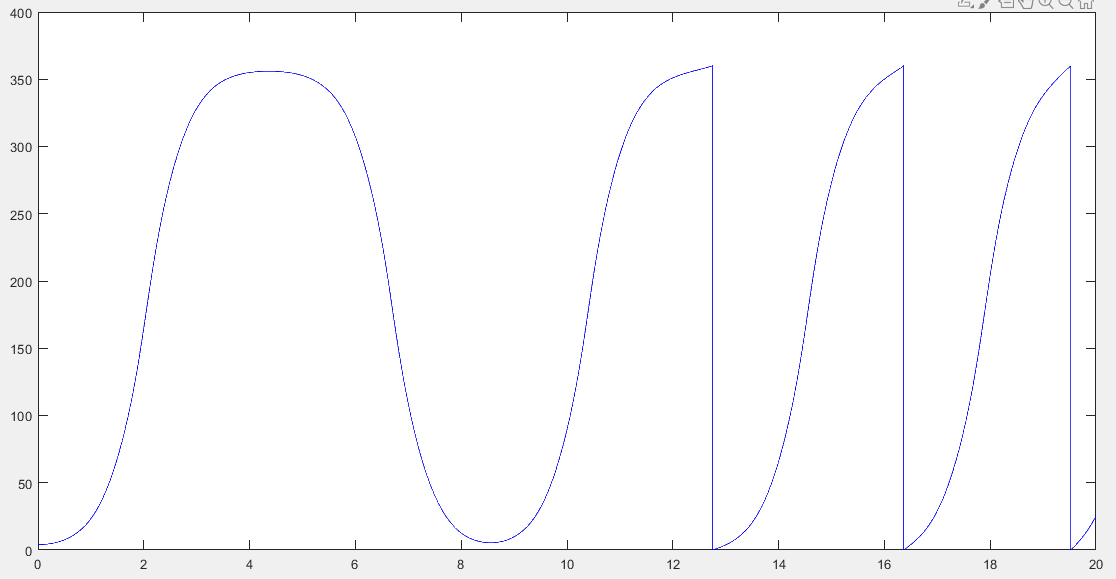
\includegraphics[width=.45\textwidth]{Immagini/open_loop_response_angle_clamped_start4deg.png}} \\
	\subfloat[][\emph{$\theta = 45deg$}]
	{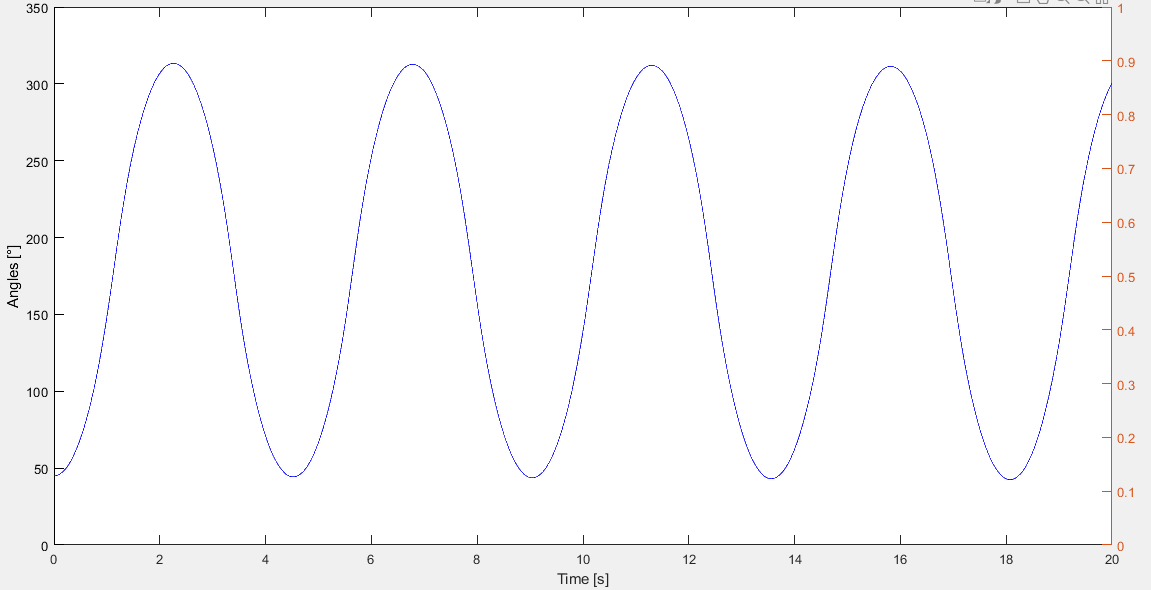
\includegraphics[width=.45\textwidth]{Immagini/open_loop_response_angle_clamped_start45deg.png}}
	\caption{Andamento angolo caratteristico $\theta$ per diversi angoli iniziali}
	\label{fig:angle_theta}
\end{figure}


La simulazione, i cui risultati sono riportati in figura \ref{fig:open_loop_response_non_linear} e \ref{fig:angle_theta}, è stata svolta per 5 e 20 secondi e con un angolo iniziale di 4°; il grafico mostra dunque l'andamento di $\theta$ nel tempo e della posizione  spaziale che, in termini matematici, si esprime come $posizione = \phi \cdot{r_{ruota}}$.

\section{Simulazione del sistema lineare}
\label{sec:simulazione_reale}
Abbiamo comunque creato, come primo step, un modello sfruttando il sistema lineare ottenuto in precedenza  con l'obbiettivo di semplificare il problema e di velocizzare le simulazioni e con lo scopo di testare rapidamente nuove tecniche di controllo che, se avessero dato esito positivo sul modello lineare, sarebbero poi state testate sul modello non lineare, che imita il comportamento reale del sistema.
\begin{figure}[H]
	\centering   	
	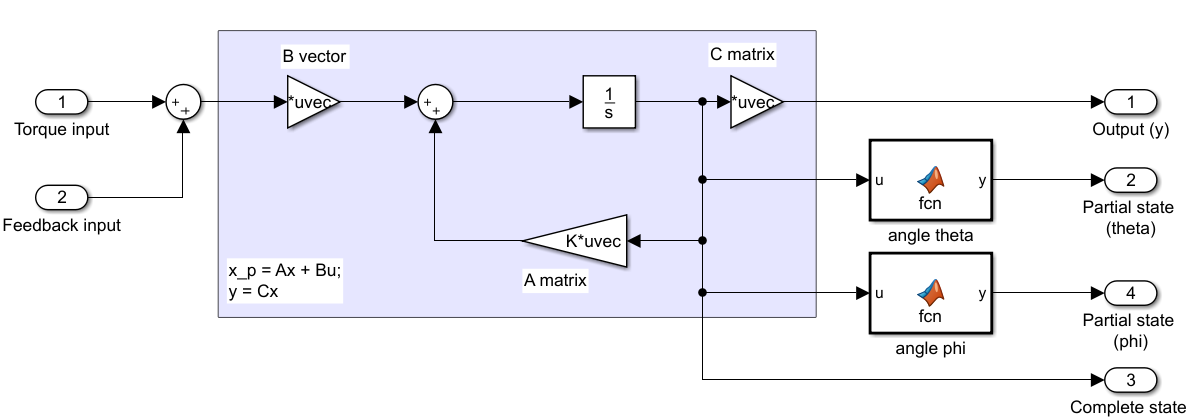
\includegraphics[width=1\textwidth]{Immagini/linear_system.png}
	\caption{Implementazione simulink del sistema linearizzato}
	\label{fig:linear_system}
\end{figure}

\begin{figure}[H]
	\centering   	
	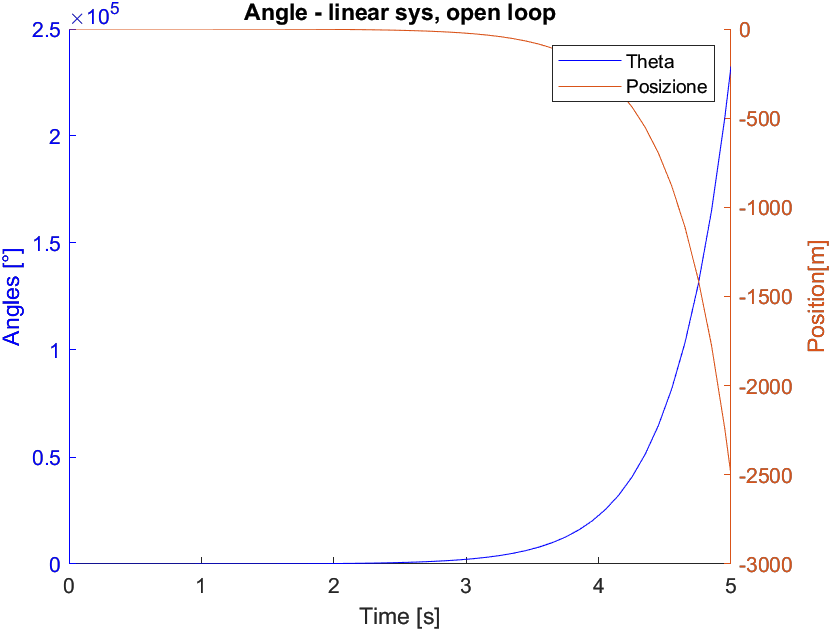
\includegraphics[width=0.6\textwidth]{Immagini/linear_open_loop.png}
	\caption{Risposta in anello aperto del sistema lineare}
	\label{fig:open_loop_response}
\end{figure}
Per completezza abbiamo comunque portato avanti la simulazione in anello aperto: il risultato ottenuto mostra che il sistema diverge.

Questo perché, come accennato in precedenza, la linearizzazione ha senso attorno al punto di equilibrio da cui è stata ottenuta, distante da quel punto il sistema lineare non approssima più il sistema reale ed anche un eventuale controllo ottenuto da esso non garantisce buone performance distante da quel punto. 

Si nota, in figura \ref{fig:open_loop_response} che il punto di partenza è di 4 deg e il sistema, lineare, diverga quasi immediatamente: la differenza con la risposta del sistema non lineare in figura \ref{fig:open_loop_response_non_linear} è lampante.


\section{Simulazione del sistema non lineare}
Il primo compito che abbiamo risolto è stato quello di implementare le equazioni differenziali ottenute nel capitolo precedente:
\begin{itemize}
	\item $\ddot{\phi} = f_{\ddot{\phi}} (M_c, C_m, \theta,\dot{\theta})$
	\item $\ddot{\theta} = f_{\ddot{\theta}} (M_c, C_m, \theta,\dot{\theta})$
\end{itemize}
Dove 
\begin{itemize}
	\item $M_c$ rappresenta la massa del passeggero;
	\item $\theta$ e $\dot{\theta}$ lo stato del sistema;
	\item $C_m$  la coppia erogata dal motore;
\end{itemize}

Si può notare come entrambe le equazioni differenziali non siano indipendenti dalla coordinata libera $\phi$.
\begin{figure}[H]
	\centering   	
	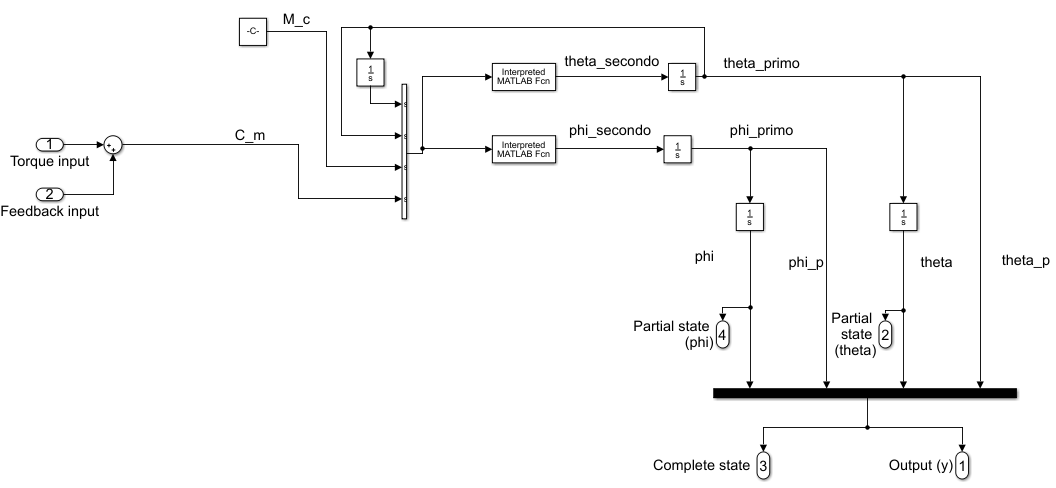
\includegraphics[width=1\textwidth]{Immagini/non_linear_system.png}
	\caption{Implementazione Simulink delle equazioni differenziali}
	\label{fig:non_linear_system}
\end{figure}

\begin{figure}[H]
	\centering   	
	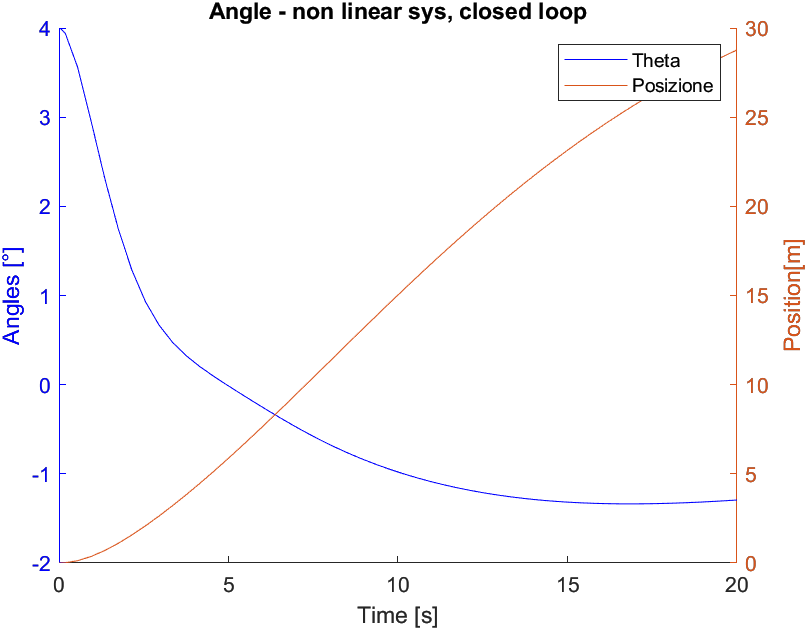
\includegraphics[width=0.7\textwidth]{Immagini/closed_loop_non_linear.png}
	\caption{Risposta del sistema non lineare in anello chiuso}
	\label{fig:closed_loop_non_linear_response}
\end{figure}

Nella figura \ref{fig:non_linear_system}, è riportata la definizione del sistema non lineare: nello specifico il core del modello è rappresentato dai blocchi \textit{interpreted function}, i quali rappresentano le funzioni  $f_{\ddot{\phi}}$ e $f_{\ddot{\theta}}$ a cui si ha fatto riferimento in precedenza.
A valle di esse sono presenti degli integratori che permettono di ottenere lo stato completo del sistema: si può facilmente notare come $\theta$ e $\dot{\theta}$ siano collegate direttamente all'input delle \textit{interpreted function} per il fatto che, come espresso dalle equazioni differenziali, si ha una dipendenza diretta da questi parametri.
Come già verificato in precedenza (sezione ~\ref{sec:open_loop_analysis}) ci sono due poli reali, uno negativo e uno positivo; questo dimostra come il sistema sia instabile in anello aperto e necessiti di controllo.

\begin{figure}[H]
	\centering   	
	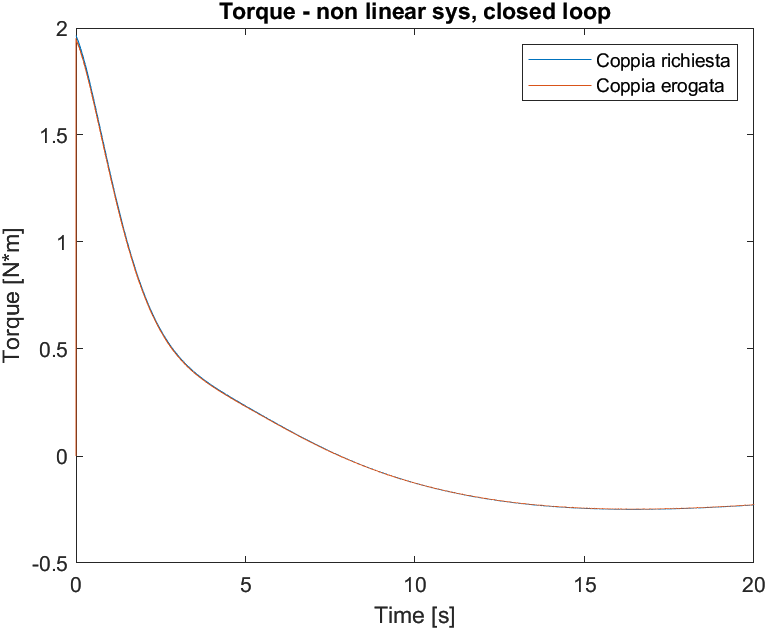
\includegraphics[width=0.7\textwidth]{Immagini/motore.png}
	\caption{Transitorio del motore}
	\label{fig:motore}
\end{figure}
\begin{figure}[H]
	\centering   	
	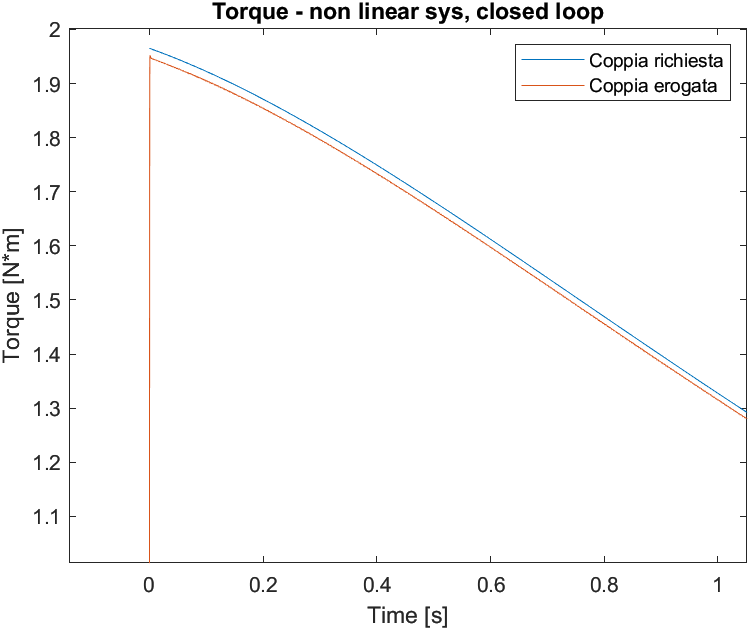
\includegraphics[width=0.7\textwidth]{Immagini/motore_zoom.png}
	\caption{Zoom del grafico in figura Fig.\ref{fig:motore}}
	\label{fig:motore_zoom}
\end{figure}

Come si può notare il picco di coppia massimo è minore di 2 Nm, come da limitazioni imposte dal modello del motore.

Un esempio in cui la coppia richiesta supera i $2N\cdot{m}$ è il seguente:
\begin{figure}[H]
	\centering   	
	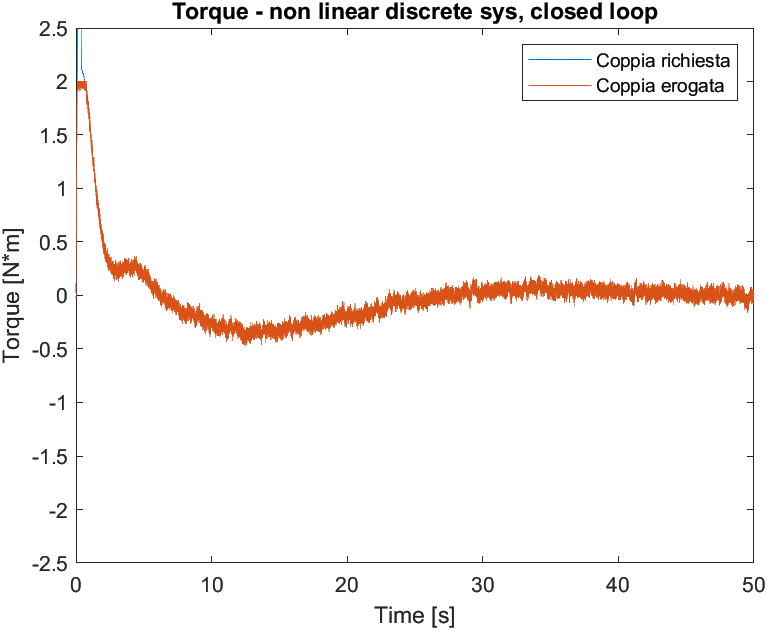
\includegraphics[width=0.7\textwidth]{Immagini/Torque.png}
	\caption{Clamp della coppia erogata da parte del motore}
	\label{fig:clamp_motore}
\end{figure}
In figura \ref{fig:clamp_motore} è anche possibile notare come l'assenza del blocchetto denominato \textit{Torque saturation}, presente in figura \ref{fig:motor}, satura l'azione integrale dell'attuatore e inserisce un ritardo non secondario nell'azione di controllo.

\section{Modello complessivo}
L'obbiettivo di questo paragrafo è quello di fare il punto della situazione del sistema sviluppato e analizzato in tutte le sue parti, riportando alcune considerazioni sul lavoro fatto.

\begin{figure}[H]
	\centering   	
	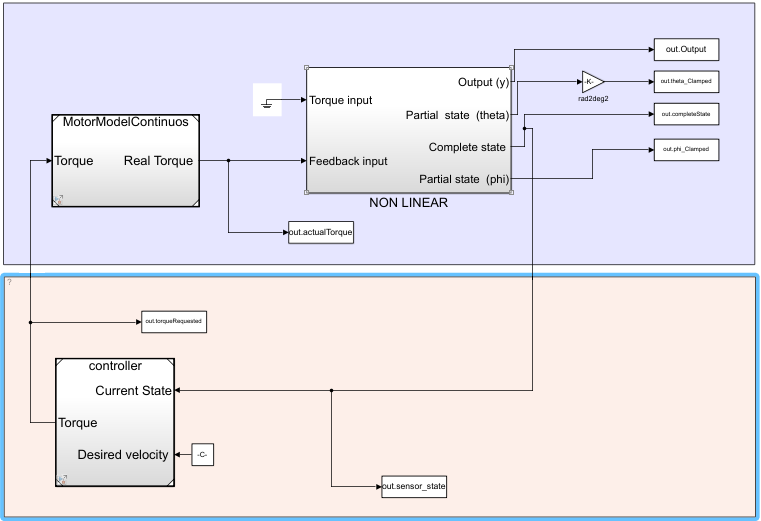
\includegraphics[width=0.8\textwidth]{Immagini/simulink_model_continuos.png}
	\caption{Modello completo}
	\label{fig:simulink}
\end{figure}
Come si osserva in figura \ref{fig:simulink} il sistema comprende quattro blocchi principali:
\begin{itemize}
	\item blocco \textit{NON LINEAR}: esso rappresenta quello che nella realtà sarebbe il sistema reale; si occupa durante la simulazione, dati gli input, di restituire output simili a quelli che si avrebbero in laboratorio utilizzando la macchina vera e propria.
	Esso è il frutto di tutto il percorso di modellizzazione mostrato nel capito ~\ref{sec:modellizzazione};
	\item blocco \textit{Sensor}: all'interno di questo blocco, siamo andati a comporre le parti necessarie per andare a filtrare e stimare lo stato del sistema, seguendo inizialmente un approccio basato su Moving Average (con un determinato valore di sliding window), passando poi ad un approccio più stabile, basato su filtraggio di Kalman;
	\item blocco \textit{controller} è, dei tre, l'unico blocco che effettivamente dovrebbe essere implementato su un calcolatore. Con i valori simulati dai due blocchi di cui sopra, esso va a calcolare il valore di coppia per il controllo e lo fornendo poi al blocco motore, completando la retroazione.
	\item blocco \textit{MotorModelDiscrete}: si occupa di simulare la presenza e i transitori dovuti ai motori posti a bordo dello chassis.
	Anche il loro funzionamento è stato discretizzato, per renderli quindi "compatibili" con quello che è il funzionamento del controllore e le letture che lo stesso processore farà delle grandezze relative agli attuatori;
\end{itemize}
Il sistema al momento è, in linea teorica, a tempo continuo. Nella realtà in un computer e in particolar modo su Simulink la possibilità di far operare i blocchi che simulano il sistema reale a tempo continuo è preclusa.
Si é scelto dunque,per quanto fatto finora, di lasciare scegliere al software di Simulink il passo della simulazione ed in particolar modo utilizzare un passo variabile. Questo permette, nei punti in cui le variazioni sono spiccate(ad esempio quando il sistema si avvia) di utilizzare un passo di simulazione anche dell'ordine dei nanosecondi che approssima quasi perfettamente l'esecuzione a tempo continuo.

\section{Discretizzazione}
Perchè discretizzare?
Come già detto sopra, il controllore è necessario che sia implementato su di un calcolatore, venendo pertanto eseguito a tempo discreto.



Per tenere conto di questa caratteristica è necessario che essa venga modellizzata in quale modo, rendendo il controllore in grado di acquisire gli input provenienti dal sistema a tempo discreto:
\begin{itemize}
	\item all'ingresso del blocco \textit{controller} è stato posto un \textit{Sample and Holder}; questo componente si occupa di acquisire ad ogni tempo di sampling $T_s$, il valore in input, campionandolo e mantenendolo inalterato fino alla lettura successiva;
	\item all'uscita del \textit{controller} si è posizionato un altro \textit{Sample and Holder} per le stesse ragioni;
	\item il \textit{controller} è stato trasformato a tempo discreto; TODO inseriamo la cosa dei poli discreti o diciamo che sono uguali essendo un proporzionale?
	A differenza del controllore della retroazione dello stato, il controllore che chiude la retroazione in velocità va ricalcolato tenendo conto del $T_s$; fortunatamente Simulink fa da solo questa conversione se si setta il blocco simulink \textit{Controllore PID} come integratore a tempo discreto fornendo il $T_s$ e la costante moltiplicativa;
	\item Tutte le \textit{grandezze fisiche} misurate sono state campionate e rese rumorose con appositi blocchi Simulink;
\end{itemize}
Il controllore a tempo discreto ha dunque questo aspetto nel modello simulink implementato:
\begin{figure}[H]
	\centering   	
	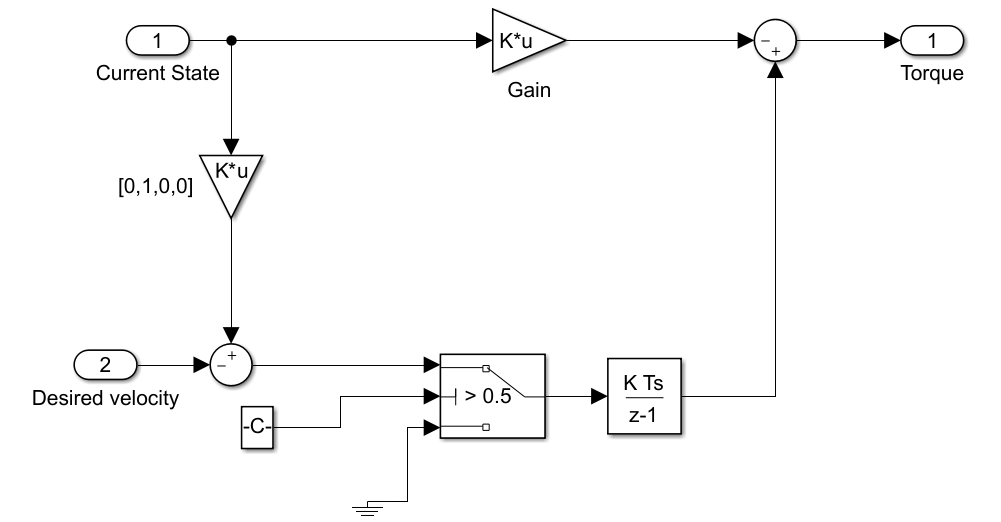
\includegraphics[width=0.8\textwidth]{Immagini/controller_discrete.png}
	\caption{Modello Simulink del controllore discreto (vista ad alto livello e vista interna)}
	\label{fig:controller_discrete}
\end{figure}

Per le stesse ragioni pratiche anche il modello del motore discreto (figura ~\ref{fig:discrete_motor}) ha subito una conversione: il controllore dell'anello di retroazione in corrente sarà un software eseguito ciclicamente su di un calcolatore e va dunque implementato a tempo discreto.
Ricordando che la funzione che la \textit{f.d.t.} del controllore \textit{PI} a tempo continuo era:
$$\dfrac{0.001216 s + 0.9965}{0.00122 s}$$
e applicando il metodo di Tustin da tempo continuo a discreto con un $T_s = 0.001$ si ottinene che:
$$\dfrac{1.037 z - 0.9557}{z - 1}$$

Quanto ottenuto a livello numerico qui sopra, è facilmente ottenibili tramite comandi per la modellizzazione dei sistemi dinamici che Matlab mette a disposizione: nello specifico, come si vede nel listato seguente, si tratta dei comandi \textit{tf} e \textit{c2d} (\textit{continous to discrete}):
\begin{lstlisting}
	PI_I = K_gi * tf([m.te,1],[m.te, 0])
	PI_I_d = c2d(PI_I,Ts,'tustin')
\end{lstlisting}

\begin{figure}[H]
	\centering   	
	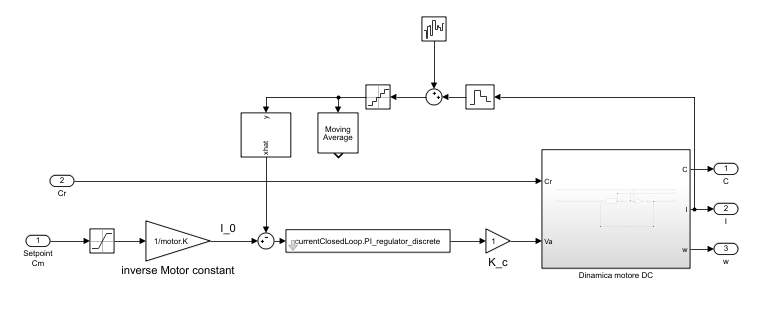
\includegraphics[width=0.8\textwidth]{Immagini/discrete_motor.png}
	\caption{Modello Simulink del motore discreto}
	\label{fig:discrete_motor}
\end{figure}

\section{Sensori}
A bordo del sistema sono presenti diversi sensori che permettono di definire e caratterizzare lo stato e il comportamento del veicolo auto bilanciato. In particolare abbiamo:
\begin{itemize}
	\item \textbf{Encoder incrementale}: si occupa di misurare la rotazione della singola ruota;
	\item \textbf{I.M.U.}: Inertial Measaurement Unit, stima l'inclinazione dello chassis;
	\item \textbf{Sensore di corrente}: permette di rilevare la corrente che fluisce all'interno del motore, per così poter realizzare un controllo in corrente dello stesso;
\end{itemize}

Questa parte di sensoristica è stata presa in considerazione con l'obbiettivo di rendere la simulazione più raffinata e accurata possibile: sono stati quindi inseriti all'interno dei file Simulink anche dei modelli che simulano la presenza dei sensori stessi.

Questo è necessario ed importante poiché nella realtà non esiste un modello matematico che genera i dati che poi sono dati in pasto al controllore ma si devono invece usare dei sensori che danno una stima dello stato del sistema. Un sensore presenta due principali caratteristiche: 
\begin{itemize}
	\item \textbf{Rumore}: è stato modellizzato come un \textit{Band-Limited
	White Noise} con \textit{Noise power} = [0.00000001] e \textit{Sample time} = 0.001 tramite lo specifico blocco Simulink;
	\begin{figure}[H]
		\centering   	
		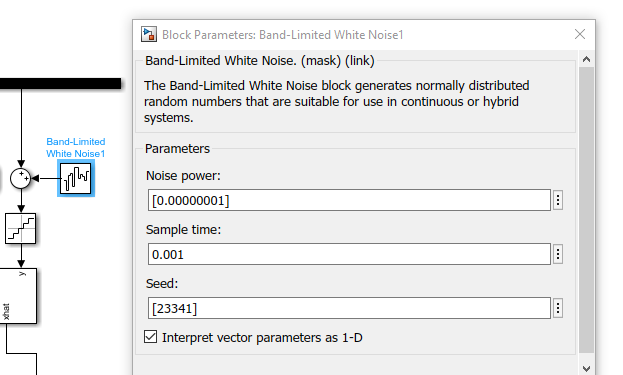
\includegraphics[width=0.5\textwidth]{Immagini/band_limited_white_noise.png}
		\caption{Blocco Simulink responsabile della generazione del rumore}
		\label{fig:band_limited_wn}
	\end{figure}
	\item \textbf{Quantizzazione}: la lettura dei dati da un sensore, oltre ad avvenire ad un intervallo di tempo minimo e regolare, mostra anche un errore dovuto alla limitata sensibilità del sensore stesso o dell' \textit{ADC} che effettua la lettura. Il blocco simulink \textit{Quantizer} ha l'esatto scopo di simulare questo comportamento presente nei sensori reali.
\end{itemize}


Per come si presenta il sistema, sia l'\textit{encoder} incrementale sia la \textit{I.M.U.} restituiscono rispettivamente una stima di $\phi$ e $\theta$
Per modellizzare quanto detto finora riguardante i sensori ed in particolare per l'\textit{encoder} e l'\textit{I.M.U.} è stato approntato il seguente blocco simulink:
\begin{figure}[H]
	\centering   	
	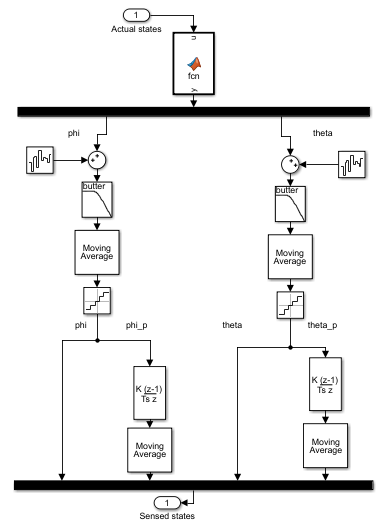
\includegraphics[width=0.6\textwidth]{Immagini/sensor_block1.png}
	\caption{Modello Simulink dei sensori \textit{encoder} e \textit{I.M.U.} con Moving Average}
	\label{fig:sensor_block1}
\end{figure}
Si può notare come in Fig.\ref{fig:sensor_block1} siano presenti due blocchi \textit{Moving average} per ciascun sensore.

Questo si è reso necessario per due ragioni:
\begin{itemize}
	\item  presentando il sistema del rumore, era necessario rimuoverlo attraverso un filtro digitale;
	\item la derivazione a tempo discreto del segnale presenta molti picchi e molti valori nulli;
	E' quindi necessario filtrare questi valori prima di passarli al controllore per evitare picchi di coppie troppo alti oppure nulli in brevi intervalli di tempo, rendendo necessario filtrare questi valori prima di passarli al controllore per evitare picchi di coppie troppo alti oppure nulli in brevi intervalli di tempo;
\end{itemize}

L'approccio con \textit{Moving average} è stato quello inizialmente seguito: abbiamo poi però cercato anche di portare avanti un altro approccio in cui, la stima dello stato, venisse effettuata tramite filtro di Kalman.
Il contesto infatti è quello in cui si ha un controllore che fornisce in uscita un comando in coppia che cambia in base allo stato del sistema $(\phi, \dot{\phi}, \theta, \dot{theta})$: i \textbf{problemi} che emergono sono però che:
\begin{itemize}
	\item $\phi$ e $\theta$ vengono misurati ma i valori forniti dai sensori sono quantizzati (quindi sarà necessario attuare un filtraggio digitalmente);
	\item $\dot{\phi}$ e $\dot{\theta}$ non sono direttamente misurabili;
\end{itemize}

Una soluzione che si è soliti seguire in contesti del genere, è quella di andare appunto ad applicare un filtro di Kalman, come già specificato, per produrre così una stima dello stato.

\begin{figure}[H]
	\centering   	
	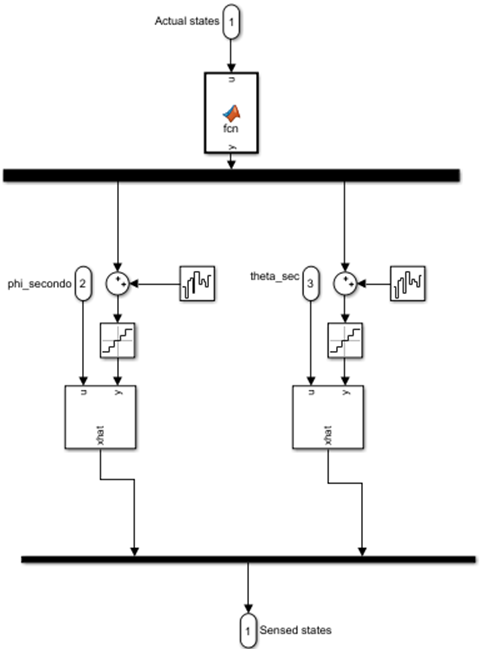
\includegraphics[width=0.6\textwidth]{Immagini/sensor_block_kalman.png}
	\caption{Modello Simulink dei sensori \textit{encoder} e \textit{I.M.U.} con Filtro di Kalman}
	\label{fig:sensor_block_kalman}
\end{figure}


Si presenta ora la necessità di modellizzare la presenza del sensore di corrente nel motore; per fare ciò si è modificato solamente l'anello di retroazione esterno che permette il controllo del motore in corrente:

Si può notare in figura \ref{fig:discrete_motor} che il controllore è quello discreto presentato prima, mentre è stato inserito anche in questo caso un rumore sulla misura, una quantizzazione e un filtro sul segnale da passare al controllore.


Da sottolineare il fatto che, ognuno dei tre blocchi \textit{Quantizer}, utilizzato per modellizzare altrattanti sensori, ha un valore diverso del parametro caratterizzante di \textit{Quantization Interval}, dovuto al fatto che ognuno dei sensori ha sensibilità diverse:
\begin{itemize}
	\item \textbf{Encoder incrementale}: presenta una sensibilità di $2^{11} bit = 2048$ diverse combinazioni e letture possibili;
	\item \textbf{I.M.U.}: sensibilità del giroscopio di $131\dfrac{s}{deg}$
	\item \textbf{Sensore di corrente}: il valore del sensore di corrente è un voltaggio letto da un Raspberry tramite ADC interno, il quale presenta sensibilità di 10 bit;
\end{itemize}